%!TEX root = ../main.tex


\begin{frame}{Redes Neurais Artificiais}
   \ \  \\[0.1cm]
  \begin{itemize}
  \item McCulloch e Pitts, 1943
  \begin{figure}[ht]
  	\centering
  	\label{fig:neuronio}
  	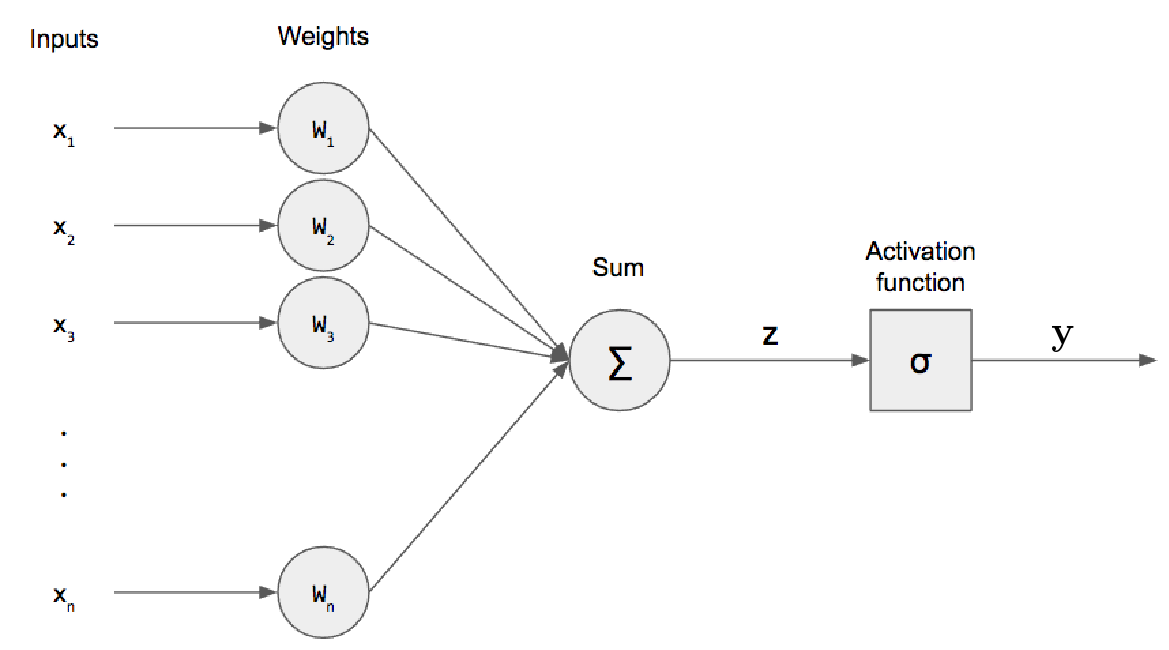
\includegraphics[width=0.7\textwidth]{img/perceptron.png}
     \caption{Representação de um neurônio artificial}
  \end{figure}
\end{itemize}
\end{frame}

\begin{frame}{Redes Neurais Convolucionais}
   \ \  \\[0.1cm]
   \begin{itemize}
     \item Topologia bem definida e estrutura em grid
    \item Destaca-se no reconhecimento de padrões em dados de alta dimensionalidade
   \end{itemize}
   \begin{figure}[!h]
   	\centering
   	\label{fig:convolutions}
   	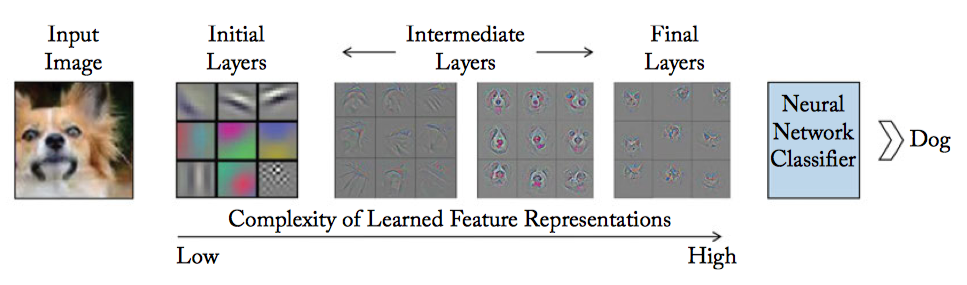
\includegraphics[width=0.8\textwidth]{./img/fundamenta/convolutions}
     \caption{Papel das camadas convolucionais e \emph{feature maps} nas CNNs.}
   \end{figure}
\end{frame}

\begin{frame}{\LARGE{Modelos Canônicos de Redes Neurais Convolucionais}}
   \ \  \\[0.1cm]
   \begin{itemize}
     \item Arquiteturas que trouxeram contribuições importantes
     \item Comuns ainda hoje no cenário de DL
     \ \ \newline
     \item LeNet (1998)
     \item AlexNet (2012)
     \item VGG (2014)
     \item Inception (2014)
     \item ResNet (2015)
     \ \ \newline
     \item \emph{Transfer Learning}: Aproveitamento de parâmetros treinados
   \end{itemize}
\end{frame}
